
Here we are going to talk about the \textbf{Dropout} method for training DL model. This is a kind of training algorithm but also a kind of parameter regularization method in some sense.


\section{Bagging and Dropout}
\begin{itemize}
	\item \textbf{Bootstrap} comes from a common saying "pull up by your own bootstraps", which means use your won resource to solve problem.
	\item \textbf{Bagging} (short for \textbf{bootstrap aggregating}) is a technique for reducing generalization error by combining several models. The idea is to train several different models separately, then have all of the models vote on the	output for test examples.This is an example of a general strategy in machine learning called	model averaging. Techniques employing this strategy are known as ensemble methods.
	\item The reason that model averaging works is that different models will usually
	not make all the same errors on the test set.
\end{itemize}
Neural networks reach a wide enough variety of solution points that they can often benefit from model averaging even if all of the models are trained on the same dataset. Differences in random initialization, random selection of minibatches,
differences in hyperparameters, or different outcomes of non-deterministic implementations of neural networks are often enough to cause different members of the ensemble to make partially independent errors.

\textbf{Dropout} provides a computationally inexpensive but	powerful method of regularizing a broad family of models. To a first approximation, dropout can be thought of as a method of making bagging practical for ensembles of very many large neural networks. Specifically, dropout trains the ensemble consisting of all sub-networks that can be formed by removing non-output units from an underlying base network.

\newpage
\begin{figure}
	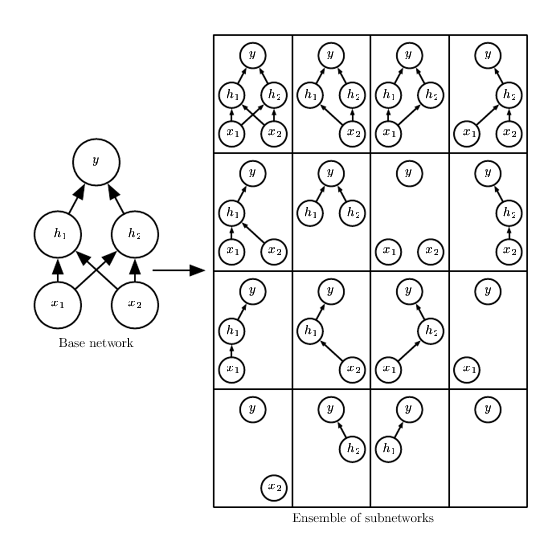
\includegraphics[width=\linewidth]{figures/dropout}
	\caption{Dropout trains an ensemble consisting of all sub-networks that can be
		constructed by removing non-output units from an underlying base network.}
	\label{fig:dropout}
\end{figure}

\begin{wrapfigure}{r}{0.4\textwidth}
	\vspace{-20pt}
	\begin{center}
		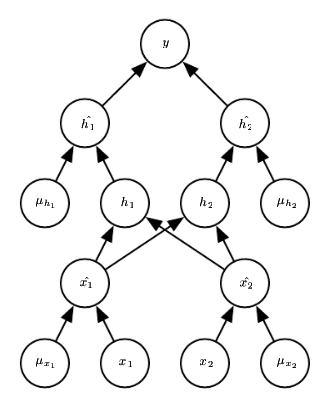
\includegraphics[width=0.38\textwidth]{figures/dropoutexample}\label{dropoutexample}
	\end{center}
	\vspace{-20pt}
	\vspace{-10pt}
\end{wrapfigure}

To perform forward propagation with dropout, we randomly sample a vector $\bm \mu$ with one entry for each input
or hidden unit in the network. The entries of $\bm \mu$ are binary and are sampled independently from each other. The probability of each entry being 1 is a hyperparameter, usually $0.5$ for the hidden layers and $0.8$ for the input. Each unit in the network is multiplied by the corresponding mask, and then forward propagation continues through the rest of the	network as usual. This is equivalent to randomly selecting one of the sub-networks from figure and running forward propagation through it.

Recall that to learn with bagging, we define $k$ different models, construct $k$ different datasets by sampling from the training set with replacement, and then train model $i$ on dataset $i$. Dropout aims to approximate this process, but with an exponentially large number of neural networks. Specifically, to train with dropout, we use a minibatch-based learning algorithm that makes small steps, such as stochastic gradient descent. Each time we load an example into a minibatch, we randomly sample a different binary mask to apply to all of the input and hidden units in the network.

Dropout training is not quite the same as bagging training. In the case of
bagging, the models are all independent. In the case of dropout, the models share
parameters, with each model inheriting a different subset of parameters from the
parent neural network. This parameter sharing makes it possible to represent an
exponential number of models with a tractable amount of memory. In the case of
bagging, each model is trained to convergence on its respective training set. In the
case of dropout, typically most models are not explicitly trained at all-usually,
the model is large enough that it would be infeasible to sample all possible sub-
networks within the lifetime of the universe. Instead, a tiny fraction of the possible
sub-networks are each trained for a single step, and the parameter sharing causes
the remaining sub-networks to arrive at good settings of the parameters. These
are the only differences. Beyond these, dropout follows the bagging algorithm.




\section{Mathematical form}

Suppose $\mathbf X=(x_1,...,x_n)$ is dataset, $\mathbf Y=(y_1,...,y_n)$ is label set. Our goal is find the parameter $\Theta=(\theta_1,...,\theta_j)$ of a neural network $f$ minimize
\begin{equation}\label{1}
\mathcal L(\Theta)=\sum_{i=1}^n L(f(x_i;\Theta),y_i)
\end{equation}
where $L(\cdot, \cdot)$ is the loss function like $L^2$ normal or cross-entropy, $f=f^j\circ\cdots\circ f^1$ is the neural network. $f^s(\mathbf x)=g(\theta_s \begin{pmatrix}
\mathbf x\\ 1
\end{pmatrix})$.

Recall the traditional Mini-Batch SGD training algorithm, for every step, we choose a subset $B_t\subset \{1,...,n\}$ and update the parameters $\Theta$ by:
\begin{equation}
\Theta^{t+1} = \Theta^t + \eta_t\nabla \sum_{i \in B_t} L(f(x_i ;\Theta) ,y_i).
\end{equation}

So the dropout means that you need to change our model just in this step, and get:
\begin{equation}
\tilde{f}^{j} = \theta^j \circ P^j \circ g^j \circ \tilde f^{j-1},
\end{equation}
with $P^j$ is a diagonal matrix for
\begin{equation}
P^j_{ii} \simeq P,
\end{equation}
with
\begin{equation}
P\{x = 0 \} = 1-\gamma_j, \quad P\{x = 1 \} = \gamma_j.
\end{equation}
and then get the update
\begin{equation}
\Theta^{t+1} = \Theta^{t} - \eta \nabla_{\Theta} \sum_{i \in B_t} L(\tilde f^J(x_i, \Theta), y_i).
\end{equation}

\subsection{Prediction}
When we finish training, we get a solution $\Theta^\#=(\theta_1^\#,...,\theta_n^\#)$.
And we can simply set the solution of \eqref{1} is $\Theta = (\gamma_1 \theta_1^\#,...,\gamma_n \theta_n^\# )$. This called \textbf{weight scaling inference rule}.
%To make the weight of each layer should be scaling to make the expectation be same as dropout.
We use a linear problem to explain this.
Suppose our problem is minimize
\begin{equation}\label{7}
\mathcal{L}(\mathbf{W})=\|\mathbf{Y}-\mathbf W\mathbf X\|_F^2
\end{equation}
so the solution of \eqref{7} $\mathbf W^*$ satisfy vanish gradient, i.e.
\begin{equation}\label{gradient}
(\mathbf Y-\mathbf W^*\mathbf X)\mathbf{X}^T=0
\end{equation}
%If $\mathbf X$ is full rank, we can get
%\begin{equation}
%\mathbf Y-\mathbf W^*\mathbf X=0
%\end{equation}


While we use dropout technology, actually we solve a series of  problems like
\begin{equation}\label{10}
\mathcal{L}(\mathbf{W})=\|\mathbf{Y}-\mathbf W(\mathbf D\mathbf X)\|_F^2
\end{equation}
where $\mathbf D=\text{diag}(\mathbf d)$, $\mathbf d$ is a random matrix with $P(d_{i}=1)=\gamma,P(d_{i}=0  )=1-\gamma$.

Its gradient is
\begin{equation}
g_t=g(\mathbf D_t)=(\mathbf Y-\mathbf W(\mathbf D_t\mathbf X))(\mathbf D_t\mathbf X)^T
\end{equation}
So the iteration step is
\begin{equation}\label{iter}
\mathbf W^{t+1}=\mathbf W^t-\eta_t g_t
\end{equation}
%We also want
%\begin{equation}
%g(\mathbf D)=\mathbf Y-\mathbf W(\mathbf D\otimes\mathbf X)=0
%\end{equation}
If \eqref{iter} is convergent, the expectation of $g$ should equals zero, so we have
\begin{eqnarray}
0=\mathbb E_{\mathbf D}(\mathbf Y-\mathbf W(\mathbf D\mathbf X))(\mathbf D\mathbf X)^T\\
=\gamma\mathbf Y\mathbf X^T-\mathbf W \gamma^2\mathbf{X}\mathbf X^T+(\gamma^2-\gamma)\mathbf W\text{diag}(\mathbf X\mathbf X^T)\\
\approx\gamma\mathbf Y\mathbf X^T-\mathbf W \gamma^2\mathbf{X}\mathbf X^T
\end{eqnarray}
So we get the solution of \eqref{10} $\mathbf W^\#$ satisfy
\begin{equation}
(\mathbf Y-\mathbf W^\#(\gamma\mathbf X))\mathbf X^T\approx 0
\end{equation}

Combine with \eqref{gradient} we can set $\mathbf W^*=\gamma\mathbf W^\#$

In other opinion,
\begin{align}
&\mathbb E_{\mathbf D}[\|\mathbf Y-\mathbf W(\mathbf D\mathbf X) \|^2_F]\\
=&\mathbb E_{\mathbf D}\text{tr}((\mathbf Y-\mathbf W \mathbf D \mathbf X)(\mathbf Y-\mathbf W \mathbf D \mathbf X)^T)\\
=&\mathbb E_{\mathbf D}\text{tr}(\mathbf Y \mathbf Y^T-\mathbf W \mathbf D \mathbf X \mathbf Y^T-\mathbf Y(\mathbf W \mathbf D \mathbf X)^T+(\mathbf W \mathbf D \mathbf X)(\mathbf W \mathbf D \mathbf X)^T)\\
=&\text{tr}(\mathbf Y \mathbf Y^T-\gamma\mathbf W \mathbf X \mathbf Y^T-\gamma \mathbf Y(\mathbf W  \mathbf X)^T+\gamma^2(\mathbf W \mathbf X)(\mathbf W  \mathbf X)^T+(\gamma-\gamma^2)\mathbf W \text{diag}(\mathbf X\mathbf X^T)\mathbf W^T )\\
=&\text{tr}((\mathbf Y-\gamma \mathbf W  \mathbf X)(\mathbf Y-\gamma \mathbf W \mathbf X)^T)+(\gamma-\gamma^2)\text{tr}(\mathbf W \text{diag}(\mathbf X\mathbf X^T)\mathbf W^T )\\
=&\|\mathbf Y-\gamma \mathbf W  \mathbf X\|^2_F+(\gamma-\gamma^2)\text{tr}( \text{diag}(\mathbf X\mathbf X^T)\mathbf W^T\mathbf W )\\
=&\|\mathbf Y-\gamma \mathbf W  \mathbf X\|^2_F+(\gamma-\gamma^2)\|(\mathbf X\mathbf X^T)^{\frac 12}\mathbf W\|_F^2\\
\end{align}
Let $ \tilde{\mathbf W}=\gamma \mathbf W$, the loss function became to 
\begin{equation}
\|\mathbf Y-\tilde{\mathbf W} \mathbf X\|^2_F+\dfrac {(1-\gamma)}\gamma\|\tilde{\mathbf W}\text{diag}(\mathbf X\mathbf X^T)^{\frac 12}\|_F^2
\end{equation}
Thus, you can think dropout for linear problem is to add a regularization term $\dfrac {(1-\gamma)}\gamma\|\tilde{\mathbf W}\text{diag}(\mathbf X\mathbf X^T)^{\frac 12}\|_F^2$.



\begin{remark}
	The analyze of linear problem only try to explain why \textbf{weight scaling inference rule} is work. It doesn't mean dropout can solve the linear problem better than not using dropout. In my(Yuyan) opinion, dropout takes the advantages of bagging method, but disadvantages of solving the problem inexactly. In most case the benefit of bagging method is greater than inexact solution. This is means the dropout has larger loss on training dataset but high accuracy on test dataset.
\end{remark}


\subsection{Inverted Dropout}


When we implement dropout, usually we use inverted dropout instead.

In tensorflow, the annotation of tf.nn.dropout shows "With probability $\gamma$, outputs the input element scaled up by $\dfrac{1}{\gamma}$, otherwise outputs 0. The scaling is so that the expected sum is unchanged."


\subsection{Numerical Experiment for Linear System}
If we consider the linear problem as a machine learning problem. We say a method is work if we get higher accuracy on test data by using this method.  Meanwhile if we consider the linear problem as a optimal problem, we say a method is work if we get less value of loss function on training dataset.


\begin{table}
	\begin{tabular}{c|c|c}
		&with dropout& without dropout\\\hline
		accuracy&86.3\%&86.3\%\\\hline
		loss &0.407&0.385\\\hline
	\end{tabular}
\end{table}
